%(Aquí lo dejaría con la estructura que teníamos para Caise, presentamos el framework y posteriormente comentamos modelos y transformaciones)

In this section we present $\pi$SOD-M, an MDD-based methodology for building service compositions with non-functional requirements. 
$\pi$SOD-M extends SOD-M with concepts for modelling non-functional requirements.
This is done at all levels of MDA, starting from the early stages of the development.
%The method uses the concept of \textit{Policy}~\cite{Espinosa-Oviedo2011a} to represent non-functional requirements.
%$\pi$-SOD-M meta-models represent both the functional aspects of the application as well as its non-functional constraints.

\begin{figure}[h]
\centering
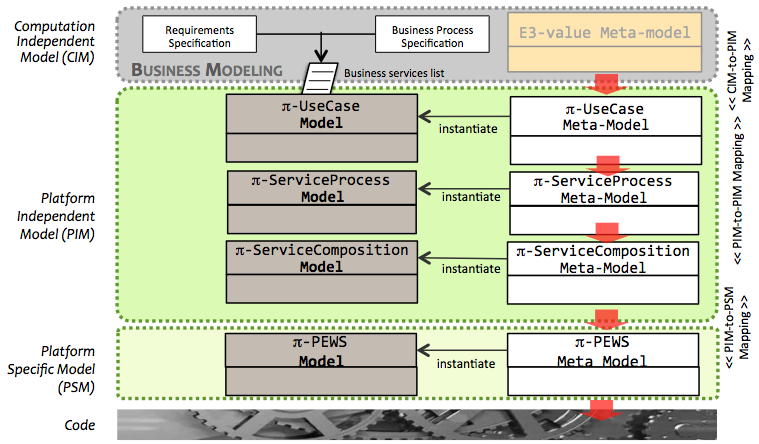
\includegraphics[width=1.0\textwidth]{figs/piSODM}
\caption{$\pi$SOD-M Overview.}
\label{fig:piSOD-M}
\end{figure}

$\pi$-SODM proposes meta-models organized into three levels (Figure~\ref{fig:piSOD-M}): 
\begin{itemize}
\item CIM (\textit{Computational Independent Models}). This level focusses on the
environment of the system, as well as on its business and requirement specifications.
This level represents the software system at its highest level of abstraction.
At this stage of the development, the structure and system processing details are still unknown or undetermined.  
$\pi$-SODM uses the \textit{e$^3$value}~\cite{e3value} and \textit{BPMN}~\cite{BPMN} meta-models for this purpose. 
%Referring to the "To Publish Music" application,  the designer starts defining an E3value model \footnote{The E3 value model is a business model that represents a business case %graphically as a set of value exchanges ($\nabla$$\triangle$) and value activities (rounded boxes) performed by business actors (squared boxes) 
%and allows  to understand the environment in which the services' composition will be placed \cite{e3value}.}  at the CIM level and then the corresponding models of the PIM are generated leading to a services' composition model (SCM).

\item PIM (\textit{Platform Independent Models}). This level focusses on the system functionality, hiding the details of any particular platform.
The specification defines those parts of the system that do not change from one platform to another. 
Our method defines three PIM-level meta-models: \textit{$\pi$-UseCase}, \textit{$\pi$-ServiceProcess} and \textit{$\pi$-ServiceComposition}.
 
 \item PSM (\textit{Platform Specific Models}). This level focusses on the functionality, in the context of a particular implementation platform.
Models at this level combine the platform-independent view with the specific aspects of the platform to implement the system. At the PSM level we have lower-level models that can be automatically translated into actual computer programs. 
We have defined one meta-model at this level.
\end{itemize}


$\pi$-SODM (Figure~\ref{fig:piSOD-M}) proposes the generation of a set of models at different levels of abstraction, as well as transformations between these models.
This can be accomplished by defining: \textit{(i)} a model-to-model transformation, from a \textit{$\pi$-ServiceComposition} model to the corresponding PSM, and \textit{(ii)} a model-to-text transformation, from the this PSM to the composition language.

The following sections describe the $\pi$-SODM meta-models, as well as the transformations between models.
The models and transformations for an industrial case are presented in section~\ref{sec:flyingPig}.

%Constraints are restrictions that must be verified during the execution of the application.
%An example of this is the requirement of the user's authentication for executing some system functions.
%


%Now, consider that besides the services' composition that represents the order in which the services are called for implementing the application "To Publish Music" it is necessary to model  other requirements that represent the (i) conditions imposed by services for being contacted, for example the fact the Facebook and Twitter require authentication protocol in order to call their methods for updating the wall; (ii) the conditions stemming from the business rules of the application logic, for example the fact that the walls in Facebook and Twitter must show the same song title and if this is not possible then none of them is updated. 
